\chapter{Umsetzung}
\label{Umsetzung}
Die Umsetzung eines Prototyps soll der Validierung des erstellten Konzepts dienen. Um das in dieser Arbeit beschriebene Konzept zu überprüfen, wurden die in \autoref{Anwendungsszenarien} beschriebenen Anwendungsszenarien, welche die Analyse und Manipulation der Netzwerkkommunikation im System ermöglichen, umgesetzt. Die Bereitstellung dieser Anwendungsszenarien erfordert aufgrund der in \autoref{Konzept:Anpassungen} beschriebenen, durch die Softwarewahl auftretenden Beschränkungen der Netzwerkkonfiguration, eine Anpassung der Architektur sowie die Erweiterung des bestehenden Systems um weitere Komponenten.

Die vorhandene Implementierung des \ac{OPC UA} Protokolls der Industrie 4.0 Testumgebung wurde um die Bereitstellung von Sicherheitsprofilen im Secure Channel erweitert. Dadurch ist es möglich, die Netzwerkkommunikation der Komponenten an der Netzwerkbrücke des Docker Services bzgl. der in \autoref{Analyse:Bedrohungen} beschriebenen Anforderungen zu analysieren. 

Des weiteren wurde das Testsystem um eine Netzwerkumgebung mit weiteren Netzwerkteilnehmern in verschiedenen Netzen erweitert. Diese stellen die Dienste DHCP sowie DNS bereit. Um die Kommunikation zwischen den Netzwerkteilnehmern und dem vorhandenen Containernetz bereitzustellen, wurde ein Router für den Transport und die Wegfindung der Pakete zwischen den verschiedenen Netzen konfiguriert. Dieser Verbund ermöglicht die Umsetzung einer \ac{MitM} Attacke mit Hilfe eines Rogue \ac{DHCP} Servers im Netzwerk.

Um den Eingriff und die Manipulation der Netzwerkkommunikation zweier Komponenten zu untersuchen, wurde eine \ac{CoAP} Client-Server Architektur implementiert. Über die beschriebene \ac{MitM} Attacke ist es möglich Informationen über die Kommunikation der implementierten \ac{CoAP} Komponenten zu erlangen und diese zu verändern.

Die Anzahl der benötigten virtuellen Komponenten wird gering gehalten, indem die vorhandenen \ac{VM}s mit mehreren Netzwerkinterfaces bereitgestellt werden. Dies ermöglicht die logische Trennung der Dienste auf einer \ac{VM} in verschiedene Netzwerke. Die Dienste werden auf die speziellen Netzwerkinterfaces gebunden. Somit kann eine Simulation der Kommunikation über Gateways ermöglicht werden.

\section{Softwarewahl}
Das Testsystem basiert auf einer Ubuntu Desktop 18.04 \ac{LTS} virtuellen Maschine und der Containervirtualisierung Docker. Beim für die Erweiterung genutzten Softwarestack wurde sich weitestgehend am Testsystem orientiert, um die Kompatibilität zu bestehenden Komponenten zu gewährleisten und weiterhin ein flexibles System bereitzustellen. Für die Analyse der Netzwerkkommunikation des genutzten Protokolls \ac{OPC UA} wurden die benötigten Änderungen direkt am Quellcode der NodeJS Implementierung des Industrie 4.0 Testsystems vorgenommen. Weitere Komponenten wurden, aufgrund von \autoref{Konzept:Anpassungen}, in weiteren virtuellen Maschinen umgesetzt, um das \ac{IPAM} des Netzwerks selbst bereitstellen und manipulieren zu können. Um Lizenzkosten zu vermeiden, wurde als Basis für die zusätzlichen virtuellen Maschinen das Betriebssystem Ubuntu Server in der letzten verfügbaren \ac{LTS} Version genutzt. Die genutzten Softwarepakete und Bibliotheken sind Bestandteil des GNU-Projekts und sollten somit analog in anderen Unix Betriebssystemen genutzt werden können. Aufgrund der weiten Verbreitung und umfangreichen Dokumentation wurde die Software \textit{isc-dhcp-server} und \textit{bind9} genutzt. Die Routingfunktionalitäten wurden über \textit{iptables} bereitgestellt. Als Hypervisor kommt weiterhin die Software "`Oracle VM Virtual Box"' zum Einsatz, um die Komplexität des Systems gering zu halten.

\section{Integration}
Die Integration des Systems beschreibt die Bereitstellung und Konfiguration der System- und Netzwerkarchitektur. Um den Zeit- und Arbeitsaufwand für die Bereitstellung des Betriebssystems zu minimieren, wurde, um die zwei zusätzlichen virtuellen Maschinen bereitzustellen, ein Minimalsystem des Ubuntu Server 18.04 (\ac{LTS}) generisch installiert und als Vorlage genutzt. Hierbei wurde der Benutzer "`i40"' mit dem Passwort "`industrie40"' angelegt, welcher für alle Maschinen gilt.

Aus der Vorlage wurden die Klone "`mgmt"' und "`comp"' erstellt. Die \ac{VM} "`mgmt"' dient der Bereitstellung der im Testnetzwerk benötigten Dienste \ac{DHCP} und \ac{DNS} und dient als Router zwischen den verschiedenen internen Netzwerken sowie zum Host System. Auf der \ac{VM} "`comp"' wurde der \ac{CoAP} Client umgesetzt. Die vorhandene \ac{VM} "`i40"' wird um einen Rogue DHCP Server erweitert. 

Zuerst wurde die Netzwerkkonfiguration aller vorhandener virtueller Maschinen wie in \autoref{Konzept:Virtuelle Maschinen} beschrieben angepasst. Dies konnte in den Einstellungen des Hypervisors durchgeführt werden. Die Netzwerkkonfiguration der \ac{VM} "`i40"' wurde von \ac{NAT} auf das interne Netzwerk "`i40-netzwerk"' geändert. Der \ac{VM} "`mgmt"' wurden drei Netzwerkadapter hinzugefügt. Der erste Adapter gehört dem internen Netzwerken "`i40-netzwerk"' an, der zweite Adapter dem internen Netzwerk "`i40-monitoring"', der dritte Adapter dient dem Host-\ac{NAT}. Die \ac{VM} "`comp"' besitzt nur einen Netzwerkadapter, welcher dem internen Netzwerk "`i40-monitoring"' angehört.

Die Installation und Konfiguration aller Komponenten sowie deren Konfigurationsdateien werden in den jeweiligen Readme Dateien des Git Repositories\footnote{GitRepository - https://github.com/fjnalta/thesis} beschrieben.

\subsection{Netzwerkverwaltung}
\label{Umsetzung:Netzwerkverwaltung}
Um die grundlegenden Netzwerkdienste in den internen Netzwerken bereitzustellen und die Kommunikation anderer Netzwerkteilnehmer mit externen Netzen wie dem Internet zur Installation und Konfiguration weiterer Software zu ermöglichen, wurde mit der Installation und Konfiguration der \ac{VM} "`mgmt"' begonnen.

Nach dem Start dem \ac{VM} wurde der Hostname zur Namensauflösung auf dem System geändert. Anschließend wurde die Netzwerkkonfiguration aller Adapter durchgeführt und den Schnittstellen der internen Netzwerke die statischen \ac{IP} Adressen 10.0.0.1 und 10.0.10.1 zugewiesen. Der Adapter zum Hostsystem bleibt unverändert. Auf der \ac{IP} Adresse 10.0.0.1 werden für das Netzwerk "`i40-network"' die Dienste \ac{DHCP} und \ac{DNS} konfiguriert. Für das Netzwerk "`i40-monitoring"' wird kein \ac{DHCP} konfiguriert, da nur zwei Komponenten im Netzwerk vorhanden sind und die Form der Adressvergabe in diesem Netzwerk keinen Einfluss auf die Umsetzung des Konzepts hat. 

\subsubsection{\ac{DNS}/\ac{DHCP}}
Eine korrekte Namensauflösung in einem Netzwerk mit dynamischen \ac{IP} Adressen kann nur ermöglicht werden, wenn die Dienste \ac{DNS} und \ac{DHCP} zusammenarbeiten. Die Authentifizierung zwischen \ac{DNS} und \ac{DHCP} zur automatischen Erstellung und Erneuerung von Zonen für Teilnehmer mit dynamischen Adressen findet mit Hilfe eines symmetrischen Schlüssels statt, welcher auf beiden Servern hinterlegt sein muss. Der Schlüssel wurde mit Hilfe des Tools \textit{rndc-confgen} erstellt.

Anschließend wurde der \ac{DNS} Server installiert und konfiguriert. Dabei wurden die Berechtigungen zum Anfragen des \ac{DNS} Servers auf das gewünschte Netz 10.0.0.0/24 beschränkt, um die Nutzung des Servers als Open \ac{DNS} zu verhindern, die \ac{DNS} Server von Google (8.8.8.8) und OpenDNS (208.67.220.220) als Forwarder genutzt, der erstellte Schlüssel eingebunden und das Interface des Dienstes auf das Netzwerk "`i40-network"' beschränkt. Auf die Konfiguration des Sicherheitsmechanismus DNSSEC wurde aus zeitlichen Gründen verzichtet.

Um eine Namensauflösung im Netzwerk bereitzustellen, wurde eine \textit{Forward-} sowie \textit{Reverselookup}-Zone für die Suchdomain "`i40-network.lan"' erstellt und die statischen \ac{IP} Adressen der \ac{VM}s "`i40"' und "`mgmt"' hinterlegt. Nach dem Neustart des Dienstes wurde mit Hilfe der Software \textit{dig} die korrekte Funktionalität der Namensauflösung im Netzwerk getestet.

Danach wurde der \ac{DHCP} Server installiert. In der Konfiguration des Servers wurde ebenfalls der erstelle Schlüssel zur Aktualisierung des \ac{DNS} Zonen hinterlegt. Es wurde das Feature "`ddns-updates"' aktiviert, den Dienst auf das Interface der Netzwerks "`i40-network"' beschränkt und die zu verteilenden \ac{DHCP} Informationen wie \ac{DHCP} Range, Gateway und Nameserver definiert. Die \ac{DHCP} Range des Servers wurde auf die Adressen 10.0.0.2 - 10.0.0.100 beschränkt, um im späteren Verlauf einen Wechsel des \ac{DHCP} Servers auf den anderen Systemen durch einen Wechsel der \ac{IP} Adresse besser verdeutlichen zu können.

Die Validierung der Funktionalität des \ac{DHCP} Servers wird durch die Konfiguration des \ac{DHCP} Clients der \ac{VM} "`comp"' durchgeführt.

\subsubsection{Routing}
Die Umsetzung der Routingfunktionalität benötigte keine zusätzliche Installation von Software. Sie wurde durch \ac{IP} Forwarding und \ac{NAT} mit Hilfe von \textit{iptables} umgesetzt. Das \ac{IP} Forwarding muss auf Betriebssystembasis durch Änderung einer Konfiguration\footnote{IPv4 Forwarding : /etc/sysctl.conf} aktiviert werden. Anschließend konnten die folgenden Regeln definiert werden, um die Pakete bei Verbindungen, welche von den internen Netzen hergestellt wurden, weiterzuleiten.

\lstinputlisting[firstline=2,language=bash,caption={Iptables},label=lst:iptables]{\srcloc/iptables.sh}

Das Interface "`enp0s3"' beschreibt die Verbindung zum Hostsystem, der Adapter "`enp0s8"' ist Teil des Netzwerks "`i40-network"', der Adapter "`enp0s9"' stellt die Schnittstelle des Routers im Netzwerk "`i40-monitoring"' dar. 

Um das Regelwerk bei jedem Neustart bereitzustellen wird es in einer Datei\footnote{iptables Konfiguration : /etc/iptables/rules.v4} gespeichert und durch das Softwarepaket \textit{iptables-persistent} bei jedem Systemstart wiederhergestellt.

\subsubsection{Delay}
Ein weiterer Bestandteil des Netzwerkstacks des Linux Kernels stellt das Tool \textit{tc}\footnote{tc - traffic control} dar. Hiermit wurde im Netzwerkinterface des \ac{DHCP} Servers ein Delay von 500ms simuliert. Dies ermöglicht im weiteren Verlauf, dass die Netzwerkpakete des Rogue \ac{DHCP} Servers früher beim anzugreifenden Client eintreffen, als die Pakete des zuständigen Servers.

\subsection{\ac{CoAP} Server}
Das Monitoringsystem der \ac{CoAP} Komponente wurde auf der \ac{VM} "`comp"' umgesetzt. Nach dem Start der Maschine wurde auch hier der Hostname angepasst und die Netzwerkkonfiguration auf \ac{DHCP} gesetzt. Dies stellte eine optimale Gelegenheit zum Testen des bereitgestellten \ac{DNS} und \ac{DHCP} Servers sowie der Routingfunktionalitäten dar.

Die Konfigurationsparameter des \ac{DHCP} Servers, welche aus \ac{IP} Adresse, \ac{DNS} und Gateway bestehen, konnten auf dem Client mit Hilfe der Tools \textit{ip} und \textit{systemd-resolv} überprüft werden und somit die korrekte Funktionalität des \ac{DHCP} Servers nachgewiesen werden. Die Funktionalität des \ac{DNS} Servers im Netzwerk konnte auf diesem Server mit dem Tool \textit{dig} nachgewiesen werden, indem die \ac{RR} der Management-\ac{VM} sowie die \ac{RR} der dynamisch bezogenen Komponenten-\ac{VM} abgefragt und überprüft wurden.

Zur späteren Ausführung des implementierten Überwachungssystems musste auf diesem System ein Webserver bereitgestellt werden. Dies geschieht durch das Paket \textit{nodejs}, welches auf dem System installiert wurde.

\section{Implementierung}
Die Implementierung umfasst die Erweiterung und Anpassung des vorhandenen Systems sowie die Bereitstellung eines neuen Dienstes. Die vorhandene Implementierung über das Protokoll \ac{OPC UA} wird angepasst, um die Kommunikation über den \textit{Secure Channel} mit Hilfe verschiedener Sicherheitsprofile zu analysieren. Hierbei wird eine unverschlüsselte sowie verschlüsselte Kommunikation zwischen \ac{OPC UA} Client und Server bereitgestellt.

Das Testsystem wurde um ein zusätzliches Monitoringsystem erweitert, welches eine \ac{CoAP} Komponente überwacht. Die Ausführung dieser Architektur dient der Analyse eines weiteren \ac{IIoT} Protokolls in Bezug auf die Manipulation von Netzwerktraffic und Verdeutlichung der Auswirkungen dieser Bedrohung.

\subsection{OPC UA Secure Channel}
\label{Umsetzung:OPC UA Secure Channel}
Um die Verwendung verschiedener Sicherheitsrichtlinien im \ac{OPC UA} \textit{Secure Channel} bereitzustellen muss die Form des Verbindungsaufbaus der vorhandenen \ac{OPC UA} Clients im Quellcode geändert werden. Die \ac{OPC UA} Server des Testsystems stellen die verschiedenen Sicherheitsprofile \textit{None}, \textit{Basic128Rsa15}, \textit{Basic256} und \textit{Basic256Sha256} bereit. Diese beinhalten den für die Nachrichtenübermittlung genutzten Verschlüsselungsalgorithmus. Bei der Übertragung der Daten im \textit{Secure Channel} wird der \ac{OPC UA} \textit{MessageSecurityMode} auf das Sicherheitsprofil angewandt. Hierbei stehen die Optionen NONE, SIGN und SIGNANDENCRYPT zur Verfügung. Im Testsystem werden keine Zertifikate verwaltet. Das Signieren der Nachrichten mit dem privaten Schlüssel des Absenders ermöglicht einen Zuwachs der Sicherheit der Netzwerkkommunikation, da dies die Integrität der Nachrichten sicherstellt. Da im Testsystem keine Verwaltung der Zertifikate stattfindet, ist kein Signieren der Nachrichten möglich. Im gegebenen System wurde jedoch die Verschlüsselung der Nachricht auf Anwendungsebene durch den Algorithmus \textit{Basic256Sha256} implementiert.

Der Quellcode der \ac{OPC UA} Clients in den Containern \textit{scheduler} und \textit{control} wurde so angepasst, dass eine Aktivierung und Deaktivierung der Verschlüsselung in der Konfigurationsdatei \textit{config.json} der jeweiligen Server vorgenommen werden kann. Zur Anwendung einer Konfigurationsänderung ist ein erneutes Bauen sowie der Neustart des Containers notwendig. Die Installation und Konfiguration der Anpassungen am bestehenden Testsystem werden in den entsprechenden Readme Dateien des Repositories beschrieben und anhand von Scripten unterstützt.

\subsection{\ac{CoAP} Monitoringsystem}
\ac{CoAP} Client und Server dienen der Repräsentation eines \ac{MitM} Angriffsszenarios. Beide Komponenten wurden mit minimaler Funktionalität implementiert. Für die Implementierung dieses Prototyps bietet sich der NodeJs Stack an, welcher mit \textit{node-coap}\footnote{node-coap - https://github.com/mcollina/node-coap} eine Bibliothek für das \ac{CoAP} Netzwerkprotokoll bereitstellt und wenig Ressourcen benötigt.

Der \ac{CoAP} Client besteht aus einem Server, welcher einen Temperatursensor einer Gießmaschine simuliert. Die Temperatur wird alle fünf Sekunden zum zuständigen Überwachungssystem übermittelt. Die Übertragung erfolgt unverschlüsselt über das Transportprotokoll \ac{UDP}, welches es möglich macht die Kommunikation im Netzwerk auch ohne Server analysieren zu können. Der Client sendet alle fünf Sekunden die Temperatur eines Sensors einer Gießmaschine zu einer in der Datei \textit{config.json} konfigurierten \ac{URL}. Der \ac{CoAP} Client wurde auf der \ac{VM} "`comp"' bereitgestellt.

Der \ac{CoAP} Server stellt den Empfänger der Nachrichten dar. Er stellt ein Webinterface bereit, um die empfangenen Daten zu visualisieren. Aufgrund der Simplizität der bereitgestellten Funktionalitäten wurde zur Implementierung des Systems ausschließlich ein \textit{Pen-and-Paper-Protoyping} durchgeführt. Der \ac{CoAP} Server bietet in der Datei \textit{config.json} die Möglichkeit die \ac{IP} Adresse, auf welche der Socket des Webservers gebunden wird zu bestimmen. Da das System auf der \ac{VM} "`mgmt"' ausgeführt wird und um dem Server im Testsystem das Netzwerk "`i40-monitoring"' zuzuweisen, wurde die \ac{IP} Adresse 10.0.10.1 in der Konfiguration gesetzt. Das \ac{GUI} des Webinterface wird in \autoref{Umsetzung:Screenshot Monitoringsystem} dargestellt.

\begin{figure}[h]
    \centering
    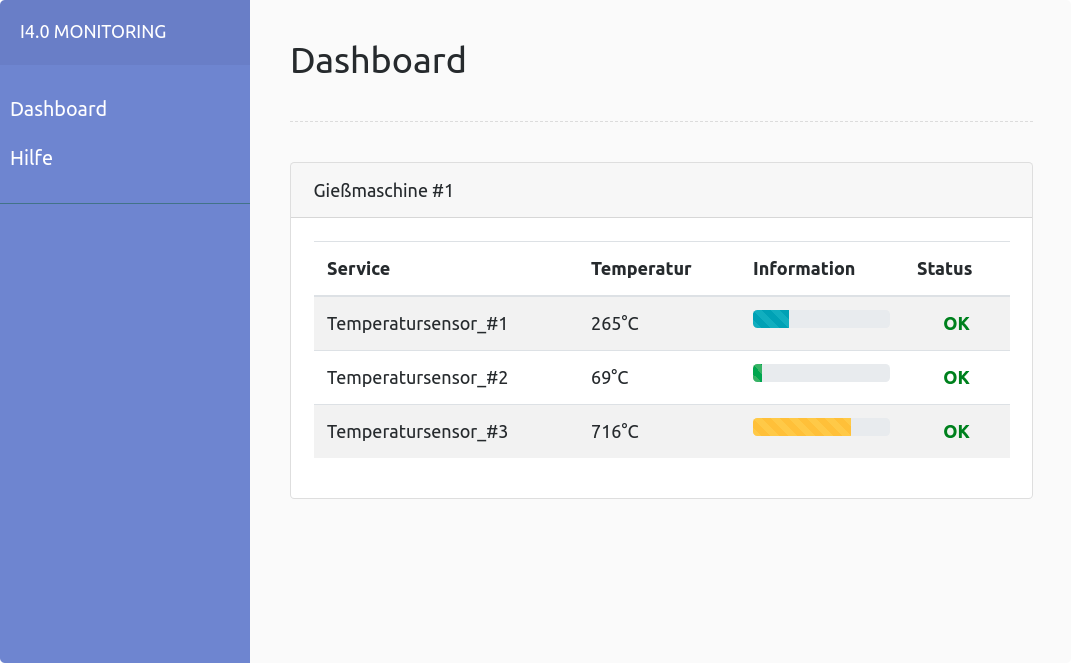
\includegraphics[width=12cm]{i40-monitoring}
    \caption{Screenshot I4.0 Monitoringsystem} 
    \label{Umsetzung:Screenshot Monitoringsystem}
\end{figure}  

\subsection{\ac{CoAP} Manipulationssystem}
Als Grundlage der Implementierung des \ac{CoAP} Manipulationssystems, diente der zuvor erstelle \ac{CoAP} Client. Dieser wurde so geändert, dass der Zielserver, der Titel der Nachricht sowie das Intervall, in welchem Daten zum Ziel gesendet werden sollen, beim Start des Servers über die Kommandozeile ermittelt werden können.

\section{Quellcode}
Der erstellte Quellcode ist im öffentlichen GitHub Repository\footnote{https://github.com/fjnalta/i40-testbed} verfügbar. Der gesamte Quellcode befindet sich im Verzeichnis "`src"' des GitHub Respositories https://github.com/fjnalta/thesis. Die Ordner "`CoAP Client"', "`CoAP Server"' und "`CoAP Manipulation"' repräsentieren die Implementierungen der \ac{CoAP} Komponenten und des Monitoringsystems. Im Ordner "`OPCUA Security Patch"' werden die aktualisierten Dateien der \ac{OPC UA} Komponenten bereitgestellt. Das genutzte Testsystem ist im Github Repository https://github.com/sneppa/i40-testbed zur Verfügung gestellt.

\section{Dokumentation}
Die Dokumentation der implementierten Komponenten, deren Inbetriebnahme und Funktionsweise findet neben der schriftlichen Ausarbeitung in den jeweiligen \textit{Readme} Dateien des Repositories https://github.com/fjnalta/thesis und dessen Unterverzeichnissen statt. Die ermöglicht die Nutzung des Testsystems auch ohne Zugang zur schriftlichen Ausarbeitung.